\section{Conclusion}

\pgfdeclareimage[width=1.0\paperwidth]{header-image}{header_images/red_lightn}
%\begin{frame}
%	\frametitle{Sensitivity to Controls}
%	%\framesubtitle{Geographic controls}
%	\begin{textblock*}{14cm}(0.3cm,1.2cm)
%		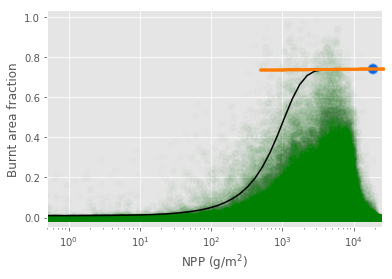
\includegraphics[width=5.78cm]{images/limitCurves/RainFsen/NPPVsFire}	
%	\end{textblock*}
%	\begin{textblock*}{14cm}(6.5cm,1.2cm)
%		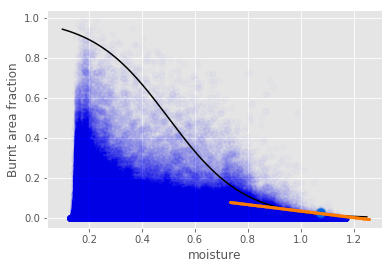
\includegraphics[width=5.78cm]{images/limitCurves/RainFsen/alphaVsFire}	
%	\end{textblock*}
%	\begin{textblock*}{14cm}(0.32cm,5cm)
%		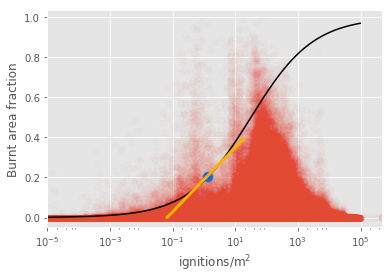
\includegraphics[width=5.78cm]{images/limitCurves/RainFsen/ignitionsVsFire.png}		
%	\end{textblock*}
%	\begin{textblock*}{14cm}(6.5cm,5.3cm)
%		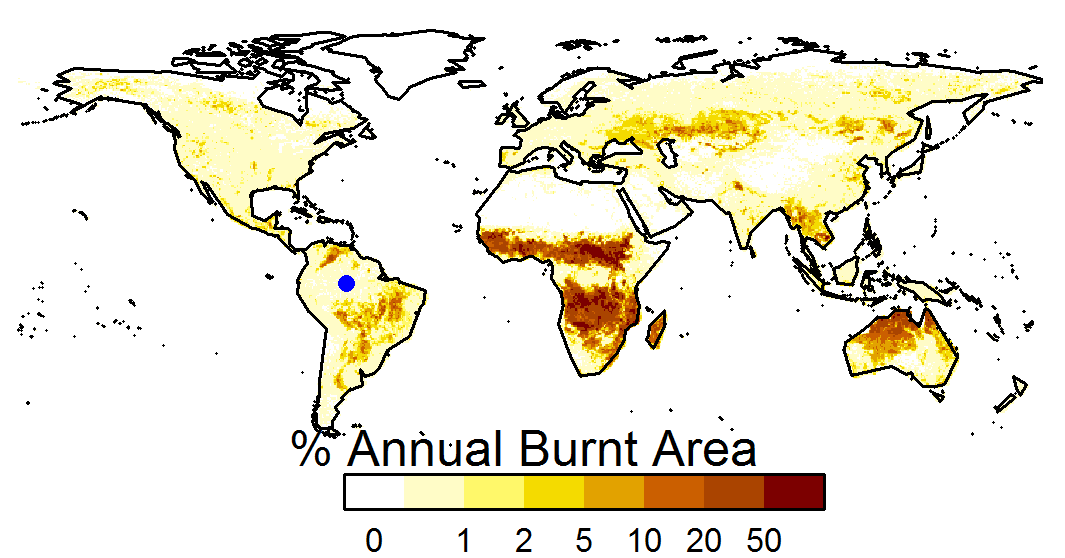
\includegraphics[width=5.78cm]{images/limitCurves/RainFsen/fireMap.png}		
%	\end{textblock*}
%\end{frame}

\addtocounter{framenumber}{-1}
%\begin{frame}<5>
%	\frametitle{Sensitivity to Controls}
%	\controlsSide{limitation_map}
%\end{frame}


\pgfdeclareimage[width=1.0\paperwidth]{header-image}{header_images/post_fire}

\begin{frame}
    \frametitle{Humans reduce burnt area}
	\begin{itemize}
		\large{
			\item Ignitions generally do not limit burnt area
			\item Human uppression have much bigger impact
            \item Cropland shows significant fragmentation affects
		}
	\end{itemize}
	\visible<2->{
		\huge{BUT...}
		\begin{itemize}
			\large{
			    \item Marginal changes in burnt area could be sensitive to changes in ignitions
				\item Human fires are a significant ignition source, particularly in pasture areas
				%\item And would likely effect other aspects of fire\\ \hspace{1cm} regime (fire size, intensity etc)
			}
		\end{itemize}
	}
\end{frame}

\begin{frame}
    \frametitle{Trends in Burnt Area}
	\begin{itemize}
		\large{
			\item Underlying shifts in burnt area controls much greater outside of tropical Savanna
			\item Boreal and tropical forests show biggest shifts
            \item from abstract
		}
    \end{itemize}
\end{frame}

\addtocounter{framenumber}{-1}
\begin{frame}
	\frametitle{Tipping points \& model assessment}
	\framesubtitle{}
	
	\begin{textblock*}{12cm}(0cm,1.5cm)
		\begin{tikzpicture}
		\node[anchor=south west,inner sep=0] (image) at (0,0) {
			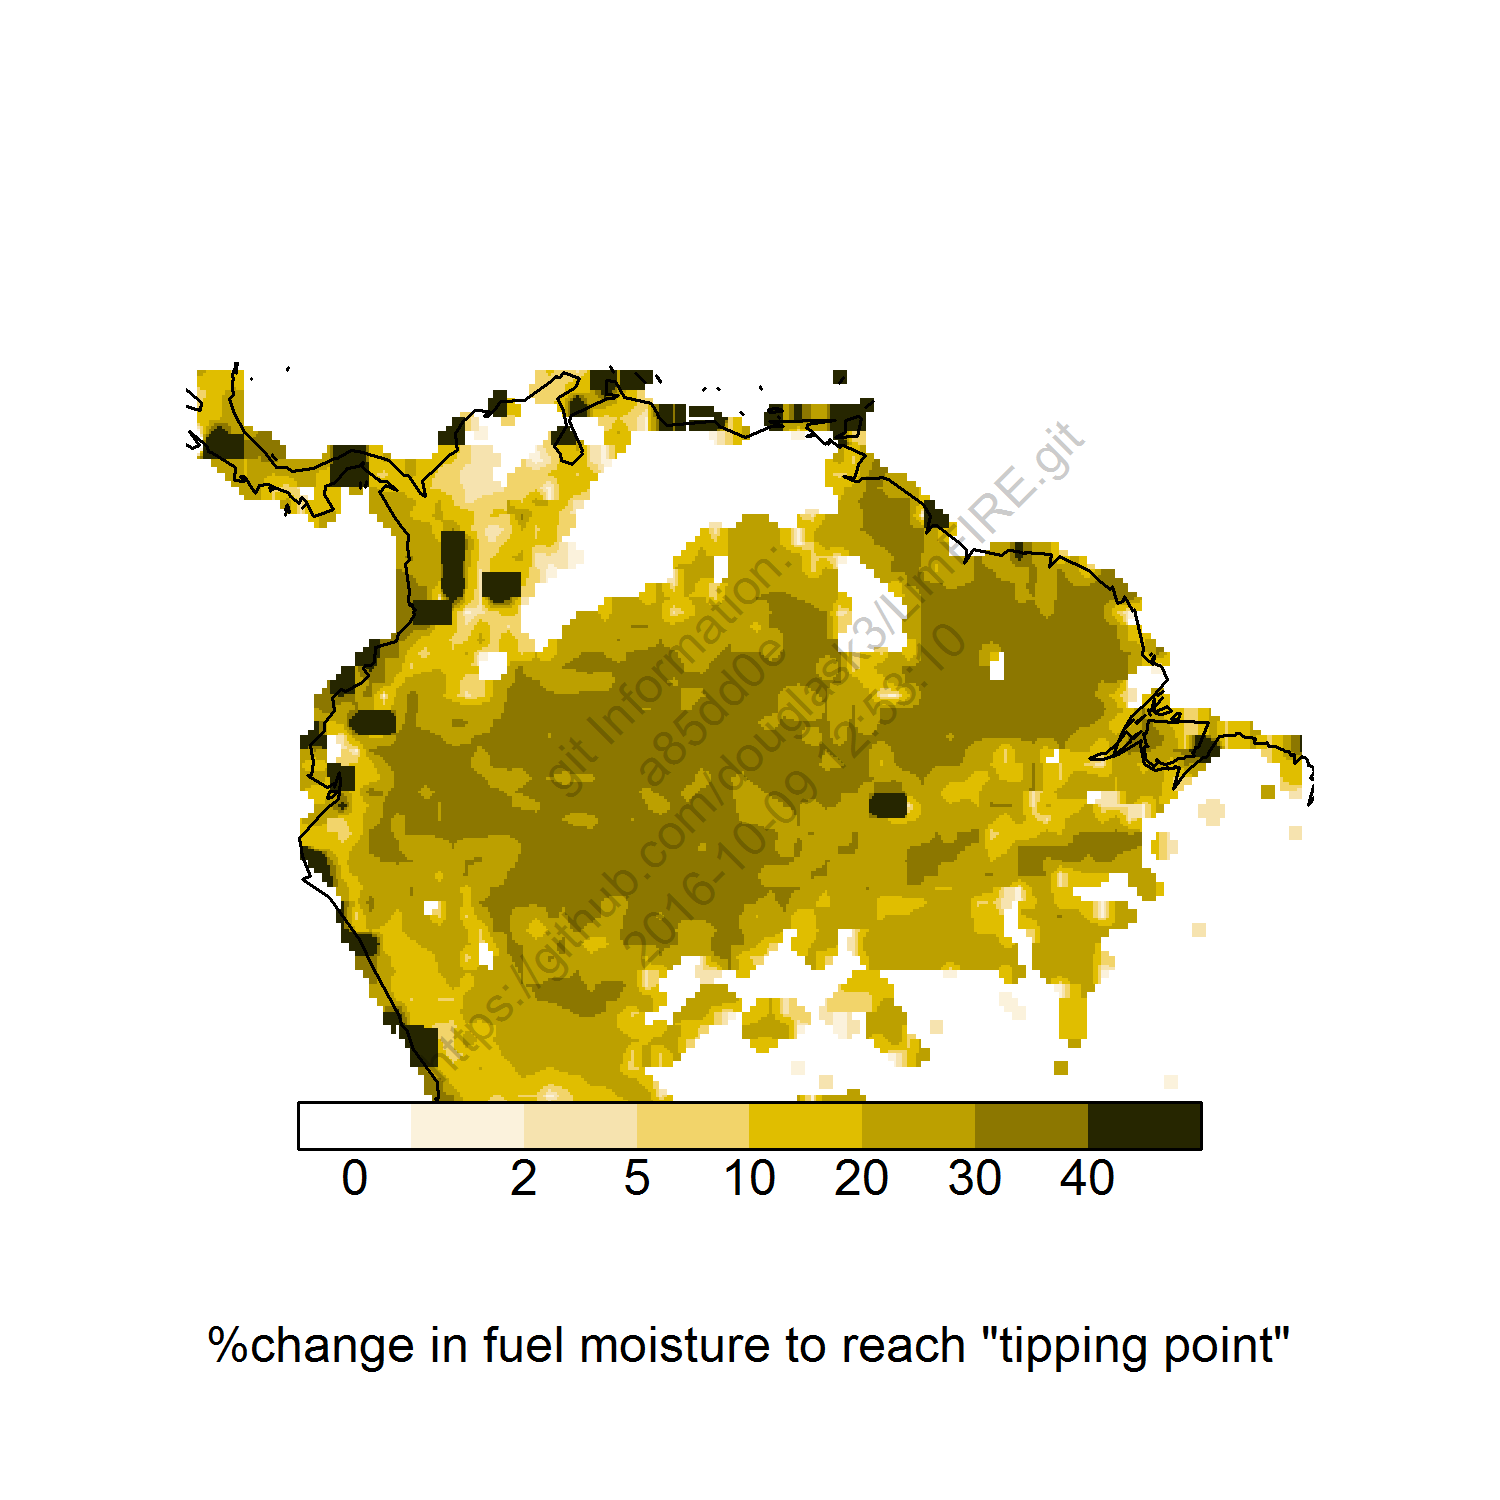
\includegraphics[width=6cm]{images/tippingPoint}
		};
		\end{tikzpicture}
	\end{textblock*}
	\begin{textblock*}{12cm}(6.5cm,1.5cm)
		\begin{tikzpicture}
		\node[anchor=south west,inner sep=0] (image) at (0,0) {
			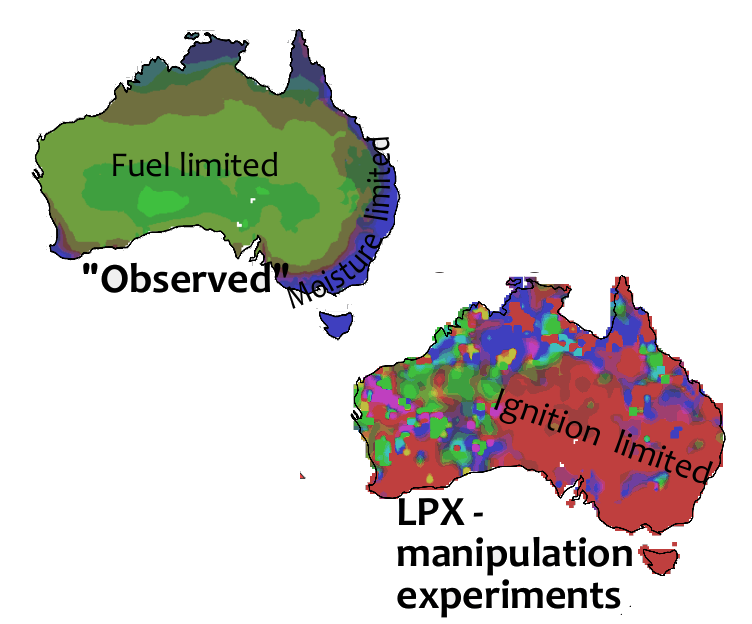
\includegraphics[width=6.0cm]{images/ModComp}
		};
		\end{tikzpicture}
	\end{textblock*}
\end{frame}

\addtocounter{framenumber}{-1}
\begin{frame}
	\frametitle{Ignitions}
	\framesubtitle{Which is more important}
	
	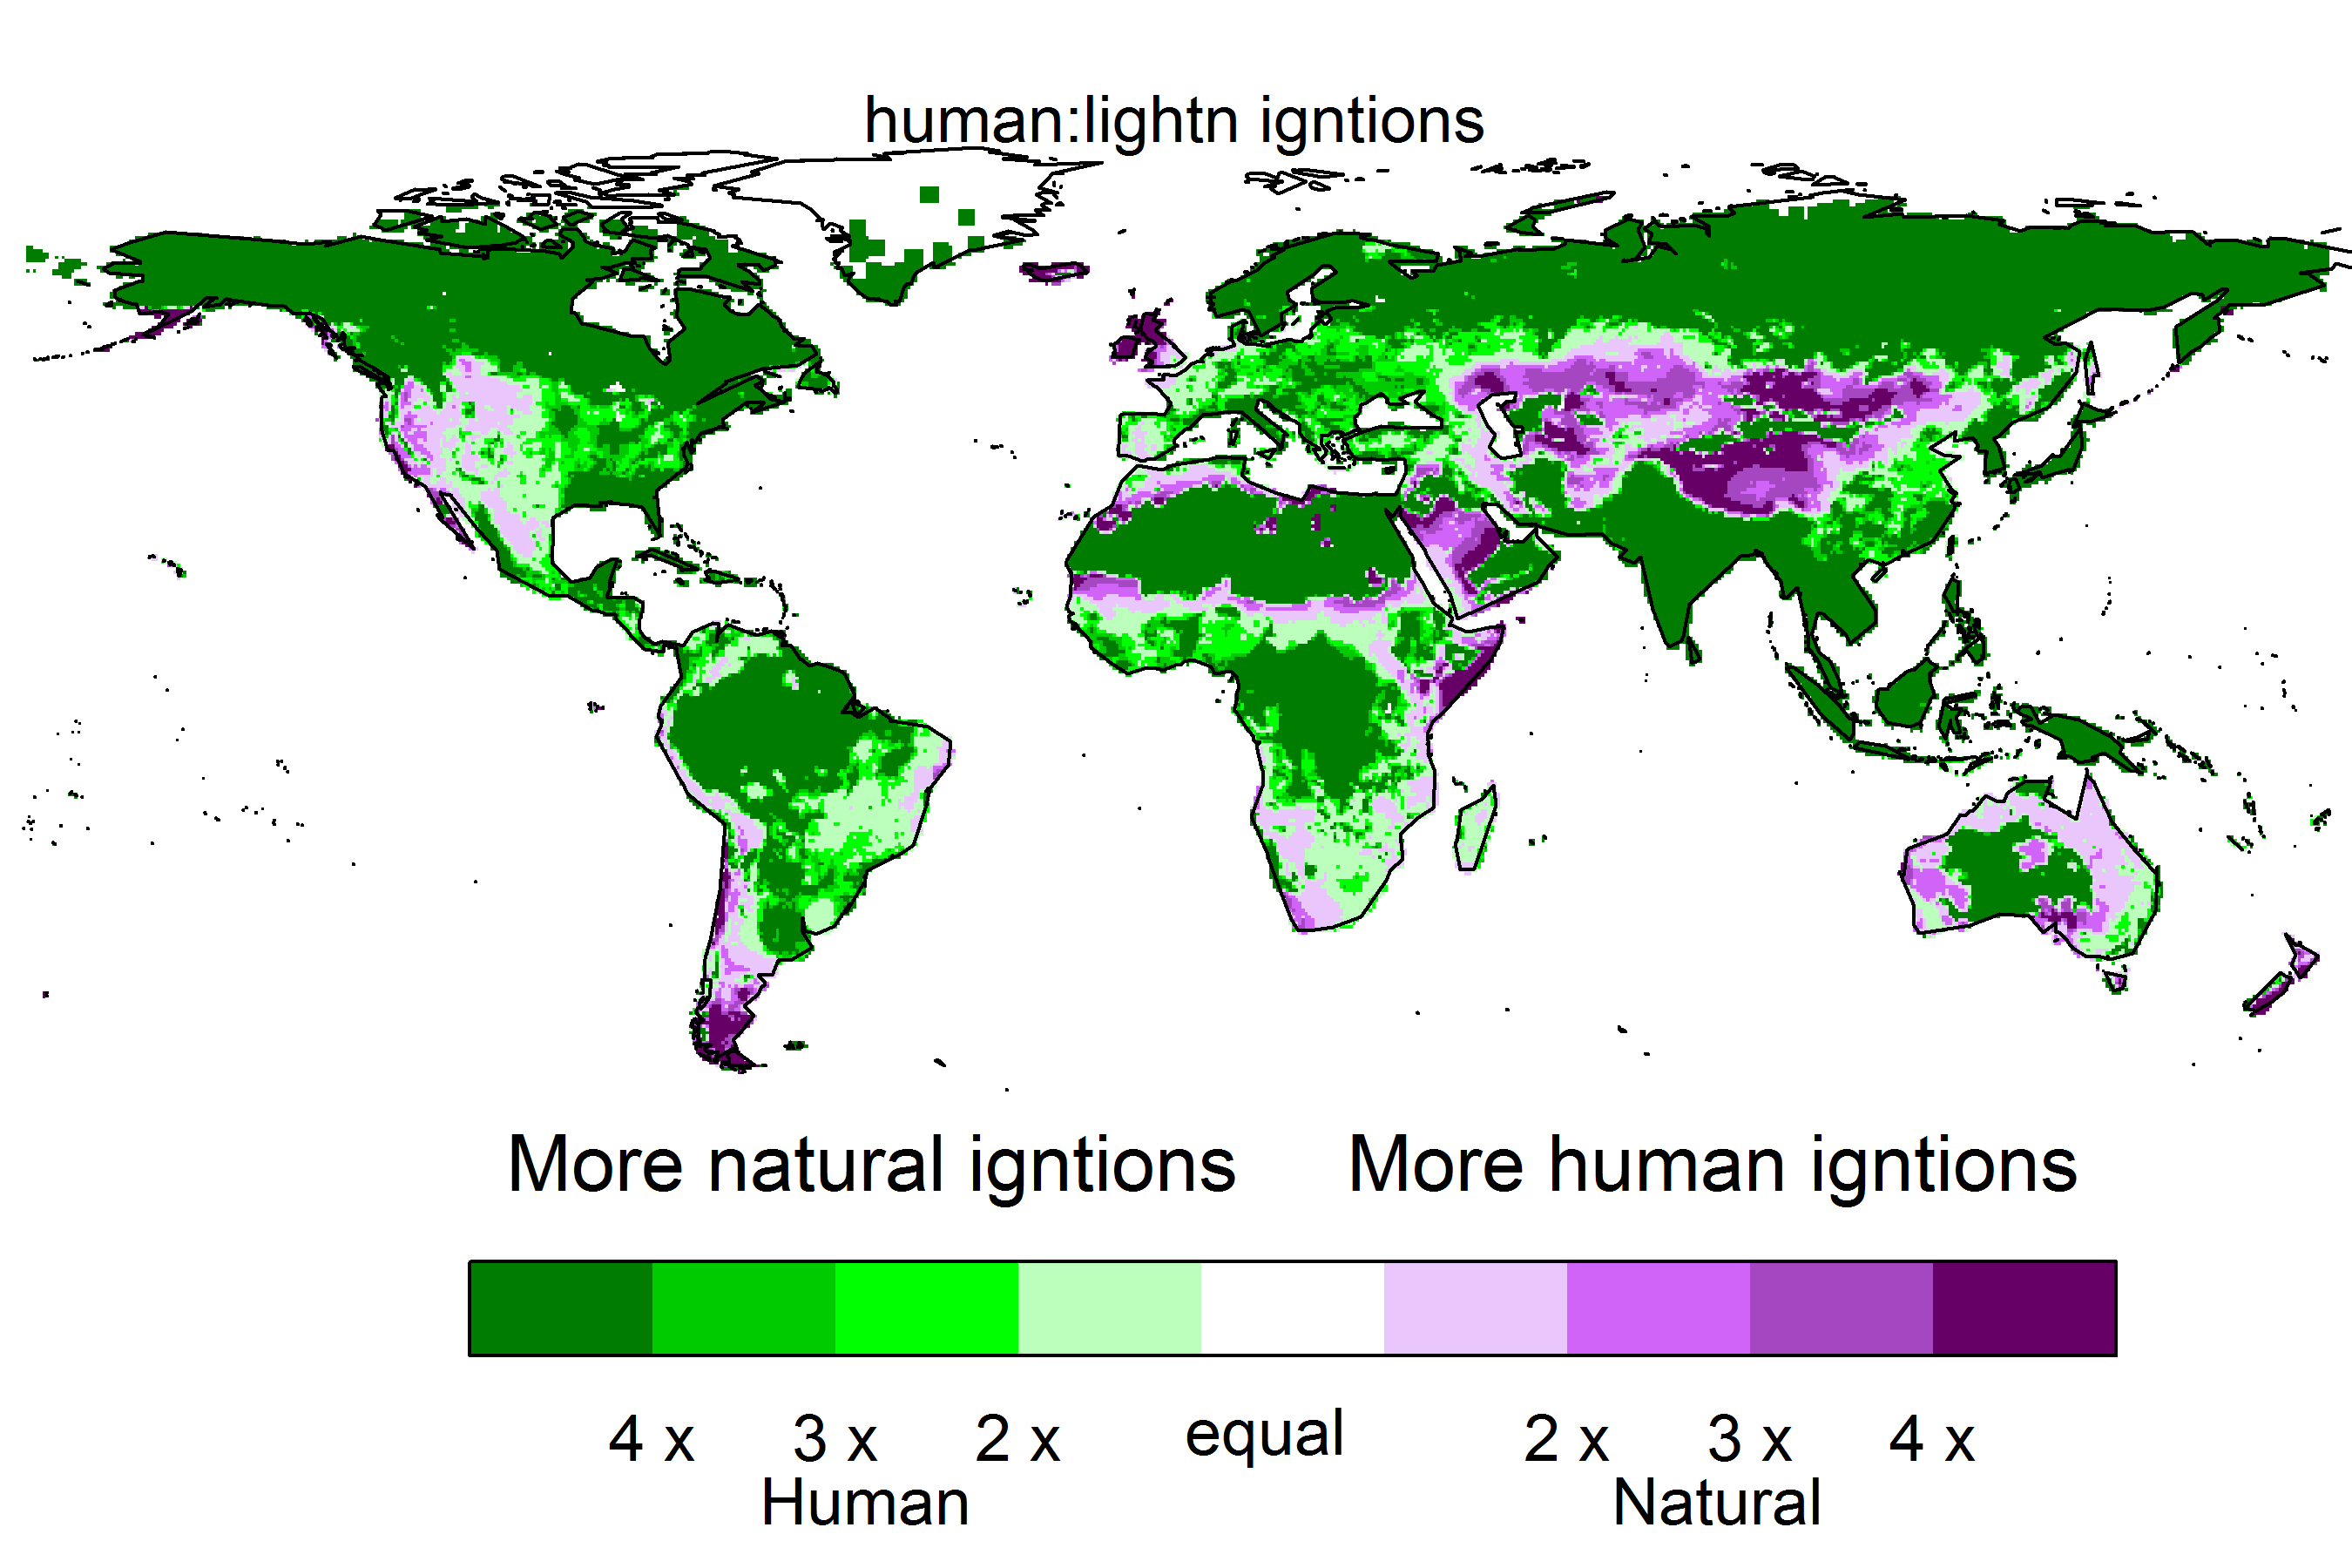
\includegraphics[width=11.0cm]{images/igntitions/IgntionInfosourceImportance}
\end{frame}


%\begin{frame}
%    \frametitle{Acknowledgments}
%    \framesubtitle{Questions..?}
%\end{frame}
